\documentclass[a4paper,12pt]{article}
\usepackage[a4paper,top=1.3cm,bottom=2cm,left=1.5cm,right=1.5cm,marginparwidth=0.75cm]{geometry}
\usepackage{cmap}
\usepackage{mathtext}
\usepackage[T2A]{fontenc}
\usepackage[utf8]{inputenc}
\usepackage[english,russian]{babel}
\usepackage{siunitx}

\usepackage{graphicx}

\usepackage{wrapfig}
\usepackage{tabularx}
\usepackage{multirow}

\usepackage{hyperref}
\usepackage[rgb]{xcolor}
\hypersetup{
colorlinks=true,urlcolor=blue
}
\usepackage{amsmath,amsfonts,amssymb,amsthm,mathtools}
\usepackage{icomma}
\mathtoolsset{showonlyrefs=false}
\usepackage{euscript}
\usepackage{mathrsfs}
\DeclareMathOperator{\sgn}{\mathop{sgn}}
\newcommand*{\hm}[1]{#1\nobreak\discretionary{}
{\hbox{$\mathsurround=0pt #1$}}{}}

%%% Заголовок
\author{Макаров Лев Евгеньевич}
\title{Лабораторная работа №2.1.6

Эффект Джоуля–Томсона
}
\date{\today}


\begin{document}

\begin{titlepage}
	\begin{center}
		{\large МОСКОВСКИЙ ФИЗИКО-ТЕХНИЧЕСКИЙ ИНСТИТУТ (НАЦИОНАЛЬНЫЙ ИССЛЕДОВАТЕЛЬСКИЙ УНИВЕРСИТЕТ)}
	\end{center}
	\begin{center}
		{\large Физтех-школа фотоники, электроники и молекулярной физики}
	\end{center}
	
	
	\vspace{4.5cm}
	{\huge
		\begin{center}
			{\bf Отчёт о выполнении лабораторной работы 2.1.6}\\
			Эффект Джоуля–Томсона
		\end{center}
	}
	\vspace{2cm}
	\begin{flushright}
		{\LARGE Автор:\\ Макаров Лев Евгеньевич \\
			\vspace{0.2cm}
			Б04-306}
	\end{flushright}
	\vspace{8cm}
	\begin{center}
		Долгопрудный 2024
	\end{center}
\end{titlepage}

\section{Введение}

\textbf{Цель работы:} 
\begin{enumerate}
	\item определить изменения температуры углекислого газа при протекании через малопроницаемую перегородку при разных начальных значениях давления и температуры
    \item вычислить по результатам опытов коэффициенты $a$ и $b$ модели Вандер-Ваальса
\end{enumerate}

\textbf{В работе используются:} 
\begin{itemize}
    \item трубка с пористой перегородкой
    \item труба Дьюара
    \item термостат жидкостной
    \item дифференциальная термопара
    \item вольтметр универсальный (мультиметр)
    \item балластный баллон
    \item манометр
\end{itemize}
\medskip

\section{Теоретические сведения}

\subsection{Теория}

Эффектом Джоуля–Томсона называется изменение температуры газа, медленно протекающего из области высокого в область низкого давления в условиях хорошей тепловой изоляции. В разреженных газах, которые приближаются по своим свойствам к идеальному газу, при таком течении температура газа не меняется. Эффект Джоуля–Томсона демонстрирует отличие исследуемого газа от идеального.

В работе исследуется изменение температуры углекислого газа при медленном его течении по трубке с пористой перегородкой (риc. \ref{ustan}). Трубка 1 хорошо теплоизолирована. Газ из области повышенного давления $ P_1 $ проходит через множество узких и длинных каналов пористой перегородки 2 в область с атмосферным давлением $ P_2 $. Перепад давления $ \Delta P = P_1 - P_2 $ из-за большого сопротивления каналов может быть заметным даже при малой скорости течения газа в трубке. Величина эффекта Джоуля–Томсона определяется по разности температуры газа до и после перегородки.

\subsection{Эффект Джоуля–Томсона}

Рассмотрим стационарный поток газа между произвольными сечениями I и II трубки (до перегородки и после нее). Пусть, для определенности, через трубку прошел 1 моль углекислого газа; $ \mu $ -- его молярная масса. Молярные объемы газа, его давления и отнесенные к молю внутренние энергии газа в сечениях I и II обозначим соответственно $ V_1, P_1, U_1 $ и $ V_2, P_2, U_2 $. Для того чтобы ввести в трубку объем $ V_1 $, над газом нужно совершить работу $ A_1 = P_1V_1 $. Проходя через сечение II, газ сам совершает работу $ A_2 = P_2V_2 $. Так как через боковые стенки не происходит ни обмена теплом, ни передачи механической энергии, то

\begin{equation}\label{1}
    A_1 - A_2 = \left( U_2 + \frac{\mu v_2^2}{2} \right) - \left( U_1 + \frac{\mu v_1^2}{2} \right)
\end{equation}

В уравнении \eqref{1} учтено изменение как внутренней (первые члены в скобках), так и кинетической (вторые члены в скобках) энергии газа. Подставляя в \eqref{1} написанные выражения для $ A_1 $ и $ A_2 $ и перегруппировывая члены, найдем

\begin{equation}\label{2}
    H_1 - H_2 = \left( U_1 + P_1 V_1 \right) - \left( U_2 + P_2 V_2 \right) = \frac{1}{2} \mu \left( v^2_2 - v^2_1 \right)
\end{equation}

Сделаем несколько замечаний. Прежде всего отметим, что в процессе Джоуля–Томсона газ испытывает в пористой перегородке существенное трение, приводящее к ее нагреву. Потери энергии на нагрев трубки в начале процесса могут быть очень существенными и сильно искажают ход явления. После того как температура трубки установится и газ станет уносить с собой все выделенное им в пробке тепло, формула \eqref{1} становится точной, если, конечно, теплоизоляция трубки достаточно хороша и не происходит утечек тепла наружу через ее стенки.

Второе замечание связано с правой частью уравнения \eqref{2}. Процесс Джоуля–Томсона в чистом виде осуществляется лишь в том случае, если правой частью можно пренебречь, т. е. если макроскопическая скорость газа с обеих сторон трубки достаточно мала. У нас сейчас нет критерия, который позволил бы установить, когда это можно сделать. В силу сохранения энтропии в случае реального газа получаем:

\begin{equation}\label{3}
    \mu_\text{Д--Т} = \frac{\Delta T}{\Delta P} \approx \frac{(2a/RT) - b}{C_P}.
\end{equation}

\subsection{Температура инверсии}

Из формулы \eqref{3} видно, что эффект Джоуля–Томсона для не очень плотного газа зависит от соотношения величин $a$ и $b$, которые оказывают противоположное влияние на знак эффекта. Если силы взаимодействия между молекулами велики, так что превалирует "поправка на давление", то основную роль играет член, содержащий $a$, и 

\[ \frac{\Delta T}{\Delta P} > 0, \]
т. е. газ при расширении охлаждается ($ \Delta T < 0 $, так как всегда $ \Delta P < 0 $). В обратном случае (малые $ a $)

\[ \frac{\Delta T}{\Delta P} < 0, \]
т. е. газ нагревается ($ \Delta T > 0 $, так как по-прежнему $ \Delta P < 0 $).

Как следует из формулы \eqref{3}, при температуре 

\begin{equation}\label{inversion-T}
    T_{\text{инв}} = \frac{2a}{Rb} 
\end{equation}

коэффициент $ \mu_\text{Д--Т} $ обращается в нуль. По формулам связи параметров газа Ван-дер-Ваальса с критическими параметрами получаем: 

\begin{equation}\label{4}
    T_\text{инв} = \frac{27}{4} T_\text{кр}.
\end{equation}

При температуре $ T_\text{инв} $ эффект Джоуля–Томсона меняет знак: ниже температуры инверсии эффект положителен ($ \mu_\text{Д--Т} > 0 $, газ охлаждается), выше $ T_\text{инв} $ эффект отрицателен ($ \mu_\text{Д--Т} < 0 $, газ нагревается).

Вернемся к влиянию правой части уравнения \eqref{2} на изменение температуры расширяющегося газа. Для этого сравним изменение температуры, происходящее вследствие эффекта Джоуля–Томсона, с изменением температуры, возникающим из-за изменения кинетической энергии газа. Увеличение кинетической энергии газа вызывает заметное и приблизительно одинаковое понижение его температуры как у реальных, так и у идеальных газов. Поэтому при оценках нет смысла пользоваться сложными формулами для газа Ван-дер-Ваальса.

Заменяя в формуле \eqref{2} $ U $ через $ C_VT $ и $ PV $ через $ RT $, найдем

\[ \left(R+C_V\right)\left(T_1-T_2\right)=\mu\left(v_2^2-v_1^2\right)/2 \]
или
\[ \Delta T = \frac{\mu}{2C_P}\left(v_2^2-v_1^2\right). \]

В условиях нашего опыта расход газа $ Q  $ на выходе из пористой перегородки не превышает $ 10 $ см$ ^3 $/с, а диаметр трубки равен 3 мм. Поэтому

\[ v_2<=\frac{4Q}{\pi d^2} = \frac{4\cdot\text{см}^3/\text{с}}{3,14\cdot(0,3)^2\text{ см}^2} \approx 140 \text{ см}/\text{с}. \]

Скорость $ v_1 $ газа у входа в пробку относится к скорости $ v_2 $ у выхода из нее как давление $ P_2 $ относится к $ P_1 $. В нашей установке $ P_1 = 4 $ атм, a $ P_2 = 1 $ атм, поэтому

\[ v_1=\frac{P_2}{P_1}v_2 = 35 \text{ см}/\text{с}. \]

Для углекислого газа $ \mu = 44 $ г/моль, $ C_P = 35,86 $ Дж/(моль·К); имеем

\[ \Delta T = \frac{\mu}{2C_P}\left(v_2^2-v_1^2\right) \approx 7\cdot10^{-4} \text{ K}. \]

Это изменение температуры ничтожно мало по сравнению с измеряемым эффектом (несколько градусов).

В данной лабораторной работе исследуется коэффициент дифференциального эффекта Джоуля–Томсона для углекислого газа. По экспериментальным результатам оценивается коэффициент теплового расширения, постоянные в уравнении Ван-дер-Ваальса и температура инверсии углекислого газа. Начальная температура газа $ T_1 $ задается термостатом. Измерения проводятся при трех температурах: комнатной, 30 $ ^\circ $C и 50 $ ^\circ $C.

\subsection{Измерение температур}

Зависимость напряжения от температурного эффекта не является линейной, поэтому необходимо использовать экспериментально полученные градуировочные кривые. В работе измеряются малые перепады температур, а для их измерения удобно использовать чувствительность термопары:

\begin{equation}
    \Delta U =\approx \frac{d U}{dt} \cdot \Delta t
\end{equation}

Обозначим чувствительность термопары за $\lambda$, тогда

\begin{equation}\label{T-from-U}
    \Delta T = \frac{1}{\lambda} \Delta U
\end{equation}


\section{Оборудование и экспериментальные погрешности}

\textbf{Вольтметр:} $\sigma_\text{V} = 0,003$ мВ \\
\textbf{Манометр:} $\sigma_\text{p} = 0,1$ атм \\
\textbf{Термометр термостата:} $\sigma_\text{T} = 0,03$ $C^\circ$ \\

Схема установки для исследования эффекта Джоуля–Томсона в углекислом газе представлена на рис. \ref{ustan}. Основным элементом установки является трубка 1 с пористой перегородкой 2, через которую пропускается исследуемый газ — двуокись углерода CO2 . Трубка имеет длину 80 мм и сделана из нержавеющей стали, обладающей, как известно, малой теплопроводностью. Диаметр трубки $d$ = 3 мм, толщина стенок 0,2 мм. Пористая перегородка расположена в конце трубки и представляет собой стеклянную пористую пробку со множеством узких и длинных каналов. Пористость и толщина пробки ($l$ = 5 мм) подобраны так, чтобы обеспечить оптимальный поток газа при перепаде давлений $\Delta P \le 4$ атм (расход газа составляет $Q \backsim 10 \ \text{см}^3/\text{с}$); при этом в результате эффекта Джоуля–Томсона создаётся достаточная для надёжного измерения разность температур.

Углекислый газ под повышенным давлением поступает в трубку через змеевик 5 из балластного баллона 6. Медный змеевик омывается водой и нагревает медленно протекающий через него газ до температуры воды в термостате. Температура воды измеряется встроенным в термостат термометром. Термостат снабжён автоматическим терморегулятором, поддерживающим постоянной температуру воды в нём с точностью $\pm 0,1 C^\circ$.

Давление газа в трубке измеряется манометром М и регулируется вентилем В (при открывании вентиля В, т. е. при повороте ручки против часовой стрелки, давление $P_1$ повышается). Манометр М измеряет разность между давлением внутри трубки и наружным (атмосферным) давлением. Так как углекислый газ после пористой перегородки выходит в область с атмосферным давлением $P_2 = P_A$, этот манометр непосредственно измеряет перепад давления на входе и на выходе трубки $|\Delta P| = P_1 - P_2$.

Разность температур газа до и после перегородки измеряется дифференциальной термопарой медь–константан. Константановая проволока диаметром 0,1 мм соединяет спаи 8 и 9, а медные проволоки (того же диаметра) подсоединены к универсальному цифровому вольтметру 7. Отвод тепла через проволоку столь малого сечения пренебрежимо мал. Для уменьшения теплоотвода трубка с пористой перегородкой помещена в трубу Дьюара 3, стенки которой посеребрены для уменьшения теплоотдачи излучением. Для уменьшения теплоотдачи за счёт конвекции один конец трубы Дьюара уплотнён кольцом 4, а другой закрыт пробкой 10 из пенопласта. Такая пробка практически не создаёт перепада давлений между внутренней полостью трубы и атмосферой.

\begin{figure}[h]
    \begin{center}$
        \begin{array}{cc}
            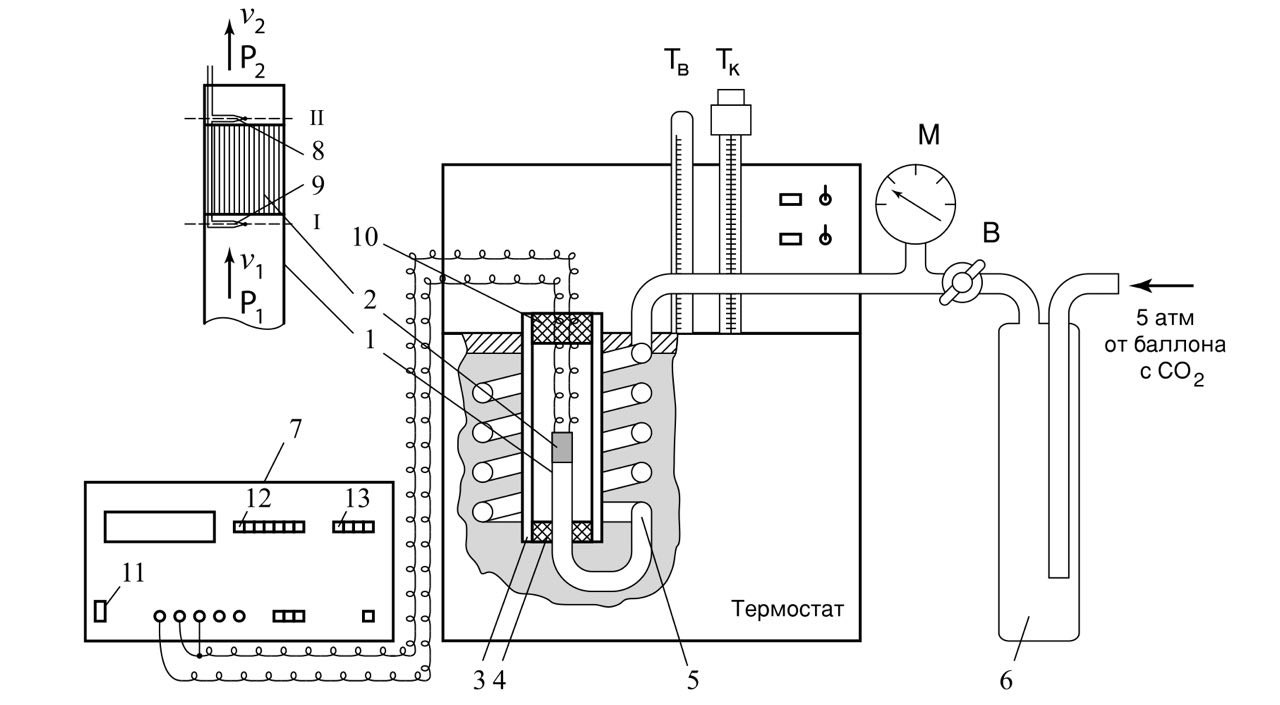
\includegraphics[width=0.8\textwidth]{ustan.png}\\
        \end{array}$
    \end{center}
    \caption{\text{Схема экспериментальной установки}}\label{ustan}
\end{figure}

\section{Результаты измерений и обработка данных}

\subsection{Проверка оборудования}

Перед началом работы убедимся, что термостат заполнен водой, а все используемые приборы заземлены.

\subsection{Подготовка термостата}

Включим термостат, установим температуру на дисплее равную $t_1 = 25 \ C^\circ$.

\subsection{Подготовка вольтметра}

Включим вольтметр и установим на нём нужный режим работы, если он не установлен.

\subsection{Предварительные измерения}

Запишем начальное показание вольтметра $U_0 = (0,005 \pm 0,003)$ мВ.

\subsection{Изучение манометра}

Цена деления манометра М составляет $\sigma_p = 0,1$ атм.

\subsection{Подготовка манометра}

Откроем регулирующий вентиль так, чтобы избыточное давление $\Delta P \approx 4$ атм. На используемой установке максимальный перепад давления составляет $\Delta P = (3,9 \pm 0,1)$ атм.

\subsection{Первоначальные измерения}

После открытия вентиля подождём 10 минут и, убедившись в том, что показания вольтметра не изменяются, запишем их в таблицу \ref{P-T-1}.

\subsection{Измерение температурного эффекта при температуре $t_1$}

При помощи вентиля В установим давление на $0,2 \backsim 0,3$ атм меньше предыидущего значения. Подождём 5 минут, пока показания вольтметра не установятся. После, запишем показания вольтметра и манометра в таблицу \ref{P-T-1}. 

Продолжим делать аналогичные измерения пока значение $\Delta P$ лежит в диапазоне от 1,5 до 4 атм. Запишем полученные измерения в таблицу \ref{P-T-1} (Сразу посчитаем значение $\Delta U$, $\sigma_{\Delta U} = 2\sigma_U$, так как $\Delta U = |U_0 - U|$). Чувствительность при данной температуре $\lambda_1 = 40,7 \ \text{мкВ}/\text{К}$. Тогда по формуле \eqref{T-from-U} посчитаем изменение температуры и запишем в таблицу \ref{P-T-1}.

\begin{table}[!h]
    \centering
    \begin{tabular}{|l|l|l|l|l|l|}
    \hline
        $N$ & $\Delta P$, атм & $U$, мВ & $\Delta U$, мВ & $\Delta T$, К & $\sigma_{\Delta T}$, К \\ \hline
        1 & 3,9 & -0,155 & 0,160 & 3,93 & 0,15 \\ \hline
        2 & 3,7 & -0,146 & 0,151 & 3,71 & 0,15 \\ \hline
        3 & 3,5 & -0,137 & 0,142 & 3,49 & 0,15 \\ \hline
        4 & 3,3 & -0,130 & 0,135 & 3,32 & 0,15 \\ \hline
        5 & 3,1 & -0,121 & 0,126 & 3,10 & 0,15 \\ \hline
        6 & 2,8 & -0,095 & 0,100 & 2,46 & 0,15 \\ \hline
        7 & 2,6 & -0,096 & 0,101 & 2,48 & 0,15 \\ \hline
        8 & 2,3 & -0,085 & 0,090 & 2,21 & 0,15 \\ \hline
        9 & 2,1 & -0,074 & 0,079 & 1,94 & 0,15 \\ \hline
        10 & 1,8 & -0,062 & 0,067 & 1,65 & 0,15 \\ \hline
        11 & 1,4 & -0,045 & 0,050 & 1,23 & 0,15 \\ \hline
    \end{tabular}\caption{\textit{Зависимость $\Delta T$ от $\Delta U$ при температуре $t_1$}}\label{P-T-1}
\end{table}

Погрешность измерения температурного эффекта $\sigma_{\Delta T} = \sigma_{\Delta U} / \lambda_1$, значение погрешности сразу запишем в таблицу \ref{P-T-1}.

\subsection{Измерение температурного эффекта при температуре $t_2$}

Повторим предыдущую серию измерений для температуры термостата $t_2 = 35 \ C^\circ$. При этой температуре чувствительность равна $\lambda_2 = 41,5 \ \text{мкВ}/\text{К}$. 

Перед началом измерений установим новую температуру и подождём 10 минут до установления равновесия. Откроем вентиль на новое $\Delta P \approx 3,4$ атм и подождём 5 минут до установления стационарного состояния. Все измерения запишем в таблицу \ref{P-T-2}.

Погрешность измерения температурного эффекта $\sigma_{\Delta T} = \sigma_{\Delta U} / \lambda_1$, значение погрешности сразу запишем в таблицу \ref{P-T-2}.

\begin{table}[!ht]
    \centering
    \begin{tabular}{|l|l|l|l|l|l|}
    \hline
        $N$ & $\Delta P$, атм & $U$, мВ & $\Delta U$, мВ & $\Delta T$, К & $\sigma_{\Delta T}$, К \\ \hline
        1 & 3,4 & -0,125 & 0,130 & 3,13 & 0,14 \\ \hline
        2 & 3,2 & -0,117 & 0,122 & 2,94 & 0,14 \\ \hline
        3 & 3,0 & -0,108 & 0,113 & 2,72 & 0,14 \\ \hline
        4 & 2,8 & -0,096 & 0,101 & 2,43 & 0,14 \\ \hline
        5 & 2,5 & -0,087 & 0,092 & 2,22 & 0,14 \\ \hline
        6 & 2,2 & -0,073 & 0,078 & 1,88 & 0,14 \\ \hline
        7 & 2,0 & -0,066 & 0,071 & 1,71 & 0,14 \\ \hline
        8 & 1,8 & -0,057 & 0,062 & 1,49 & 0,14 \\ \hline
    \end{tabular}\caption{\textit{Зависимость $\Delta T$ от $\Delta U$ при температуре $t_2$}}\label{P-T-2}
\end{table}

\subsection{Построение графика}

Построим график зависимости $\Delta T$ от $\Delta P$ для двух серий измерений. Для этого воспользуемся МНК для апроксимации наилучшей прямой. В данном случае $v = \Delta P$, а $u = \Delta T$. Так как зависимость должна быть линейной, то

\begin{equation}
    k = \frac{\langle uv\rangle - \langle u \rangle \langle v \rangle}{\langle v^2 \rangle - \langle v \rangle^2},
    \ \text{а} \ \  b = \langle u \rangle - k\langle v \rangle
\end{equation}

Погрешности для $k$ и $b$ рассчитываются по формулам:

\begin{equation}
    \sigma_k = \frac{1}{\sqrt{n}} \sqrt{\frac{\langle u^2 \rangle - \langle u \rangle^2}{\langle v^2 \rangle - \langle v \rangle^2} - k^2}
\end{equation}

\begin{equation}
    \sigma_b = \sigma_k\sqrt{\langle v^2 \rangle - \langle v \rangle^2}
\end{equation}

Пользуясь этими формулами посчитаем $k$ и $b$ для двух серий измерений, а также коэффициенты Джоуля-Томсона:

\begin{equation}
    \mu_1 = k_1 = (1,09 \pm 0,03) \ \frac{\text{К}}{\text{атм}} \ \ \ b_1 = (-0,34 \pm 0,03) \ \text{К}
\end{equation}

\begin{equation}
    \mu_1 = k_2 = (1,02 \pm 0,02) \ \frac{\text{К}}{\text{атм}} \ \ \ b_1 = (-0,35 \pm 0,01) \ \text{К}
\end{equation}

Экспериментальные точки и апроксимированные прямые нанесём на график \ref{graph}.

Табличные значения коэффициентов при данных температурах лежат в диапазоне от 1,02 до 1,11 К/атм. А значит экспериментальные значения с хорошей точностью совпадают с табличными.


\subsection{Определение постоянных $a$ и $b$ в модели Ван-дер-Ваальса}

Для нахождения $a$ и $b$ воспользуемся соотношением \eqref{3}:

\begin{equation}
    \mu_i = \frac{(2a/RT_i) - b}{C_P} = \frac{2a}{R C_P} \left( T_i \right)^{-1} - \frac{b}{C_P}
\end{equation}

Отсюда следует, что

\begin{equation}
    a = \frac{R C_P}{2} \frac{\mu_1 - \mu_2}{\left( T_1 \right)^{-1} - \left( T_2 \right)^{-1}} = \frac{8,31 \cdot 35,86(1,09 - 1,02)}{2 ((298,26)^{-1} - (308,16)^{-1})} = 0,9 \ \frac{\text{Дж} \cdot \text{м}^3}{\text{моль}^2}
\end{equation}

Погрешность $a$ можно вычислить по формуле:

\begin{multline*}
    \sigma_a = \sqrt{
    \left ( \frac{\partial a}{\partial \mu_1} \right )^2 \sigma_{\mu_1} ^ 2 +
    \left ( \frac{\partial a}{\partial \mu_2} \right )^2 \sigma_{\mu_2} ^ 2 +
    \left ( \frac{\partial a}{\partial T_1} \right )^2 \sigma_{T_1} ^ 2 +
    \left ( \frac{\partial a}{\partial T_2} \right )^2 \sigma_{T_2} ^ 2
    } = \\
    = \frac{R C_P}{2} \sqrt{
    \frac{\sigma_{\mu_1}^2 + \sigma_{\mu_2}^2}{\left( \left( T_1 \right)^{-1} - \left( T_2 \right)^{-1} \right)^2} + 
    \left( 
    \frac{\left( \mu_1 - \mu_2 \right)^2}{\left( \left( T_1 \right)^{-1} - \left( T_2 \right)^{-1} \right)^4}
    \right) \left( \frac{\sigma_{T_1}^2}{T_1^4} + \frac{\sigma_{T_2}^2}{T_2^4}\right)
    } = \\
    = a \sqrt{
    \frac{\sigma_{\mu_1}^2 + \sigma_{\mu_2}^2}{\left( \mu_1 - \mu_2 \right)^2} + 
    \frac{\frac{\sigma_{T_1}^2}{T_1^4} + \frac{\sigma_{T_2}^2}{T_2^4}}{\left( \left( T_1 \right)^{-1} - \left( T_2 \right)^{-1} \right)^2}
    }
\end{multline*}

\begin{equation}
    \sigma_a = 0.9 \sqrt{
    \frac{0,03^2 + 0,02^2}{\left( 1,09 - 1,02 \right)^2} + 
    \frac{\frac{0,03^2}{298,26^4} + \frac{0,03^2}{308,16^4}}{\left( 298,26^{-1} - 308,16^{-1} \right)^2}
    } = 0,5 \ \frac{\text{Дж} \cdot \text{м}^3}{\text{моль}^2}
\end{equation}

Теперь $b$ можно найти по формуле:

\begin{equation}
    b = \frac{2a}{R T_1} - \mu_1 C_P = \frac{2 \cdot 0,9}{8,31 \cdot 298,16} - 1,09 \cdot 10^{-5} \cdot 35,86 = 37 \cdot 10^{-5} \ \frac{\text{м}^3}{\text{моль}}
\end{equation}

Погрешность вычисления $b$ можно найти по формуле:

\begin{multline*}
    \sigma_b = \sqrt{
    \left ( \frac{\partial b}{\partial a} \right )^2 \sigma_{a} ^ 2 +
    \left ( \frac{\partial b}{\partial T_1} \right )^2 \sigma_{T_!} ^ 2 +
    \left ( \frac{\partial b}{\partial \mu_1} \right )^2 \sigma_{\mu_1} ^ 2
    } = \\
    = \sqrt{
    \left( \frac{2}{R T_1} \right)^2 \sigma_{a} ^ 2 + 
    \left( \frac{2 a}{R T_1^2} \right)^2 \sigma_{T_1} ^ 2 + C_P^2 \sigma_{\mu_1} ^ 2
    } = \\
    = \frac{2 a}{R T_1} \sqrt{
    \frac{\sigma_a^2}{a^2} + \frac{\sigma_{T_1}^2}{T_1^2} + \left( \frac{R T_1 C_P \sigma_{\mu_1}}{2 a} \right)^2
    }
\end{multline*}

\begin{equation}
    \sigma_b = \frac{2 \cdot 0,9}{8,31 \cdot 298,26} \sqrt{
    \frac{0,5^2}{0,9^2} + \frac{0,03^2}{298,26^2} + \left( \frac{8,31 \cdot 298,26 \cdot 35,86 \cdot 0,03}{2 \cdot 0,9} \right)^2
    } = 1 \cdot 10^{-5} \ \frac{\text{м}^3}{\text{моль}}
\end{equation}

Оценим температуру $T_\text{инв}$, пользуясь соотношением \eqref{inversion-T}:

\begin{equation}
    T_\text{инв} = \frac{2 a}{R b} = \frac{2 \cdot 0,9}{8,31 \cdot 0,00037} = 612 \ \text{К}
\end{equation}

Погрешность вычисления $T_\text{инв}$ можно вычислить по формуле:

\begin{equation}
    \sigma_{T_\text{инв}} = T_\text{инв} \sqrt{
    \left( \frac{\sigma_a}{a} \right)^2 + \left( \frac{\sigma_b}{b} \right)^2
    } = 612 \sqrt{
    \left( \frac{0,5}{0,9} \right)^2 + \left( \frac{1}{37} \right)^2
    } = 342 \ \text{К}
\end{equation}

Запишем табличные величины и экспериментальные в таблицу \ref{comp}.

\begin{table}[!ht]
    \centering
    \begin{tabular}{|l|l|l|}
    \hline
        ~ & эксп & табл \\ \hline
        $a$, $\text{Дж} \cdot \text{м}^3 / \text{моль}^2$ & 0,9 & 0,36 \\ \hline
        $b$, $10^{-5} \text{м}^3/\text{моль}$ & 37 & 4,2 \\ \hline
        $T_\text{инв}$, К & 612 & 2053 \\ \hline
    \end{tabular}\caption{\textit{Сравнение табличных величин с экспериментальными}}\label{comp}
\end{table}

Видно, что табличные значения сильно отличаются от экспериментальных.

\section{Обсуждение результатов и выводы}

В ходе работы был измерен температурный эффект углекислого газа при протекании через малопроницаемую перегородку, а также вычислены коэффициенты $a$ и $b$ модели Вандер-Ваальса.

Однако, полученные экспериментально значения сильно разняться с табличными и погрешность их вычисления велика. Это можно объяснить большим количеством упрощений и приближений, использовавшихся для получения формулы \eqref{3}. также ошибка велика из-за того, что коэффициенты Джоуля-Томсона вычислялись всего по двум сериям измерений, а значит $a$ и $b$ вычислялись по двум точкам.

Из этого можно сделать вывод, что данная модель не подходит для измерения и объяснения эффекта Джоуля-Томсона.

\newpage


\begin{figure}[h!]
        \centering
	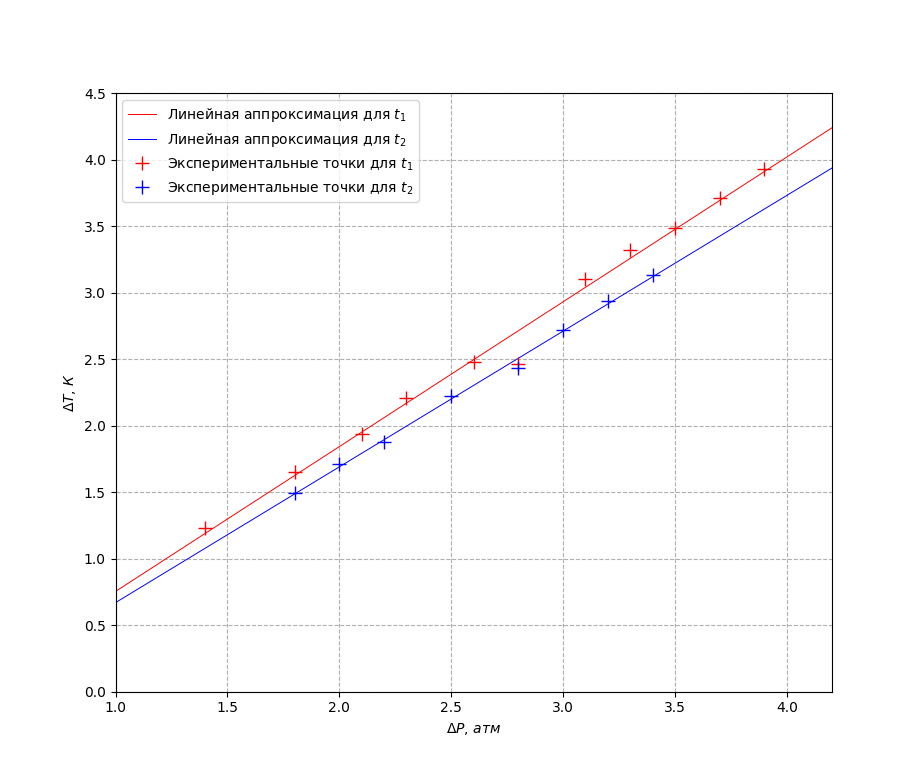
\includegraphics[width=1.1\textwidth]{graph.png}
	\caption{\textit{График зависимости $\Delta T$ от $\Delta P$ для обоих наборов измерений}}
	\label{graph}
\end{figure}

\end{document}